\section{Levi-Civita and the Geometry of Transport: From Algebra to Parallelism}

If Ricci built the algebra of curvature,  
then Tullio Levi-Civita gave that algebra its geometric soul.

Where Ricci’s tensor calculus provided a symbolic machinery for curvature,  
Levi-Civita asked:

\begin{quote}
“What does it mean to move a vector along a curve in a curved space?”
\end{quote}

And from that question arose a breakthrough:  
the notion of **parallel transport**—a rule for moving vectors along a path while keeping them “as parallel as possible,” even as the space beneath them bends.

\bigskip

\subsection*{The Leap from Ricci to Levi-Civita}

Ricci’s tensors encoded curvature algebraically,  
capturing how coordinate systems twisted and how derivatives had to be corrected.

But Levi-Civita saw that Ricci’s Christoffel symbols weren’t merely correction terms—  
they defined a **connection**: a geometric structure that told you how to “connect” vectors at infinitesimally separated points.

Where Ricci saw tensors as algebraic objects,  
Levi-Civita saw them as describing the behavior of vectors under transport.

✅ How does a vector “point in the same direction” as it moves through curved space?  
✅ How can you define “straightness” when Euclidean lines no longer apply?

Levi-Civita’s answer was to formalize **parallel transport**:  
the process of moving a vector along a curve so that its covariant derivative vanishes:

\[
\nabla_{\dot{\gamma}} V = 0
\]

Here, \( \nabla \) is the **covariant derivative**, and \( \dot{\gamma} \) is the tangent vector to the curve.

This equation encodes that \( V \) is “transported parallelly” along \( \gamma \).

\bigskip

\begin{tcolorbox}[colback=gray!5!white, colframe=black, title=\textbf{Sidebar: The Shift from Ricci to Levi-Civita}, fonttitle=\bfseries, arc=1.5mm, boxrule=0.4pt]

\begin{tabular}{>{\raggedright}p{4cm} >{\raggedright}p{5.5cm} >{\raggedright\arraybackslash}p{5.5cm}}
 & \textbf{Ricci} & \textbf{Levi-Civita} \\
\midrule
Key contribution & Tensor calculus to encode curvature algebraically & Geometric interpretation of how vectors move in curved spaces \\
Focus & Curvature expressed as tensors & Parallel transport and covariant differentiation \\
Key tool & Riemann curvature tensor; Ricci tensor & Affine connection; Levi-Civita connection (torsion-free, metric-compatible)
\end{tabular}

\end{tcolorbox}

\bigskip

\subsection*{From Algebraic Encoding to Geometric Meaning}

Where Ricci gave the algebra to compute curvature,  
Levi-Civita gave a geometric process to experience it.

Parallel transport provided a way to visualize curvature:

✅ Move a vector around a closed loop,  
✅ Bring it back to where it started,  
✅ Observe how it “rotated” simply by moving through space.

This rotation wasn’t caused by an external force—  
it was an intrinsic property of the space itself.

\bigskip

In Levi-Civita’s connection, Ricci’s symbols acquired **operational meaning**:  
they weren’t just components of formulas,  
they told you how geometry itself guided vectors as they moved.

Levi-Civita’s formulation also guaranteed two key properties:

✅ The connection was **torsion-free**: moving along different paths yields consistent outcomes.  
✅ The connection was **metric-compatible**: parallel transport preserves inner products (length and angles).

\bigskip

\begin{quote}
In Euler, we computed forces.  
In Lagrange, we minimized action.  
In Hamilton, we traced flows.  
In Jacobi, we found surfaces.  
In Cayley, we abstracted transformations.  
In Fourier, we decomposed vibrations.  
In Riemann, we curved the space.  
In Gibbs, we calculated fields.  
In Peano, we defined the space.  
In Christoffel, we corrected differentiation.  
In Ricci, we encoded curvature.  
In Levi-Civita, we learned how to move inside curvature.
\end{quote}

\subsection*{The Geometry Ready for Physics}

With Levi-Civita’s connection, geometry wasn’t just a static fabric;  
it was a space through which vectors could move, paths could bend, and curvature could be experienced dynamically.

This connection made it possible to define **geodesics** as curves whose tangent vectors are parallel transported along themselves.

It provided the geometric machinery needed not just to describe curvature,  
but to calculate how objects move in a curved space.

And it gave Einstein, just a few years later, the last mathematical tool he needed:  
a way to write the laws of gravity as the geometry of spacetime itself.


\subsection*{Reinterpreting Kepler’s Second Law Through Levi-Civita’s Parallel Transport}

Kepler’s Second Law tells us that a planet sweeps out equal areas in equal times.  
In earlier frameworks, this became:

\begin{itemize}
    \item Conservation of angular momentum (Gibbs),
    \item Invariance under rotational symmetry (Ricci),
    \item Preservation of areal velocity via covariant derivatives (Christoffel).
\end{itemize}

But Levi-Civita gave this conservation law a deeper geometric meaning:  
it is a statement about how vectors move along a curved path in such a way that they remain “as parallel as possible.”

\bigskip

\paragraph{Parallel Transport Along an Orbit.}

Let \( \gamma(t) \) be the worldline of the planet — a curve through a curved space (or spacetime).  
Let \( \vec{L}(t) = \vec{r}(t) \times \vec{v}(t) \) be the angular momentum vector.

Kepler’s Second Law asserts that the direction and magnitude of \( \vec{L}(t) \) remain constant.

In Levi-Civita’s language, this is expressed as:

\[
\nabla_{\dot{\gamma}} \vec{L} = 0
\]

That is: \( \vec{L} \) is **parallel transported** along the orbit.  
It does not rotate or change in magnitude when moved via the Levi-Civita connection.

\bigskip

\paragraph{From Conservation to Curvature-Invariant Motion.}

In flat space, this reduces to ordinary vector constancy.  
But in curved space, it means:

\begin{itemize}
    \item The orbit respects the geometry of the space,
    \item The geometry preserves certain symmetries (e.g., rotation),
    \item Those symmetries ensure that certain vectors — like angular momentum — are preserved under parallel transport.
\end{itemize}

Thus, Kepler’s Law is not just a classical remnant —  
it is a **geometric consequence of parallel transport in a symmetric, curved manifold**.

\bigskip

\begin{tcolorbox}[colback=blue!5!white, colframe=blue!80!black, title=\textbf{Levi-Civita’s Take on Kepler}]
Kepler saw areas.  
Newton saw forces.  
Levi-Civita saw a vector that moves with the curve,  
obeying the geometry, never twisting against it.
\end{tcolorbox}

\begin{figure}[H]
    \centering
    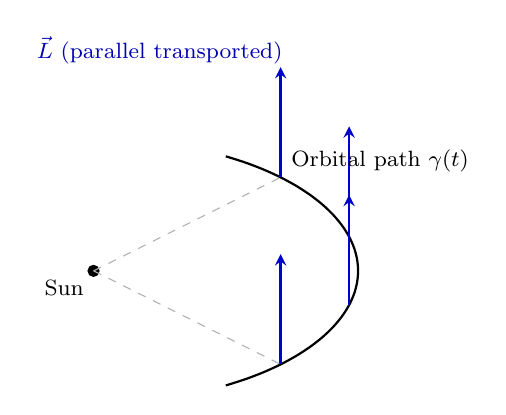
\begin{tikzpicture}[scale=2.8, >=stealth]
    
    % Central mass (Sun)
    \filldraw[black] (0,0) circle (0.025) node[below left] {\footnotesize Sun};
    
    % Elliptical orbit arc
    \draw[thick, domain=-60:60, smooth, variable=\t] 
      plot ({1.2*cos(\t)}, {0.6*sin(\t)});
    
    % Angular momentum vectors (parallel transport arrows)
    \foreach \angle in {-45,-15,15,45} {
      \draw[->, thick, blue!80!black]
        ({1.2*cos(\angle)}, {0.6*sin(\angle)})
        -- ++(0,0.5);
    }
    
    % Labels on vectors
    \node[blue!70!black] at (0.3,1.0) {\footnotesize $\vec{L}$ (parallel transported)};
    
    % Radial vectors to show position (optional)
    \draw[dashed, gray!60] (0,0) -- ({1.2*cos(-45)}, {0.6*sin(-45)});
    \draw[dashed, gray!60] (0,0) -- ({1.2*cos(45)}, {0.6*sin(45)});
    
    % Curve label
    \node at (1.3,0.5) {\footnotesize Orbital path $\gamma(t)$};
    
    \end{tikzpicture}
    \caption{Levi-Civita’s interpretation of Kepler’s Second Law: the angular momentum vector \( \vec{L} \) is parallel transported along the orbital path \( \gamma(t) \), maintaining its direction and magnitude in accordance with the Levi-Civita connection.}
    \end{figure}
    